\newpage
\section{Regression}
%\begin{figure}[H]
%  \centering
%  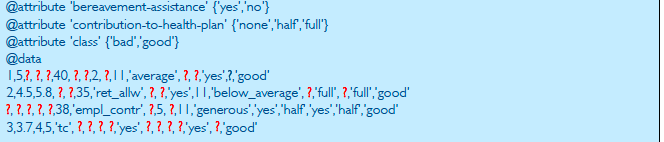
\includegraphics[width=.5\linewidth]{arffmissing}
%\end{figure}
Regression can be summarized as 
$$ \text{Regression = model building + model usage}$$
Given N examples , pairs $x_i,y_i$,  \textbf{linear regression} computes a model $$y = w_0 + w_1x $$ so that for each point $$ y_i = w_0 + w_1x_i + \epsilon_i$$
The model is evaluated using $$ RSS(w_0,w_1)= \sum \limits_{i=1}^{N} (y_i-(w_0+w_1x_i))^2$$ and the goal for linear regression is to \textbf{minimize the RSS} by finding the right weights : 
$$ w_0,w_1 = arg min_{w_0,w_1} RSS(w_0,w_1)=arg min_{w_0,w_1}\sum \limits_{i=1}^{N} (y_i-(w_0+w_1x_i))^2 $$
To minimize those weights :
\begin{enumerate}
\item Set \textbf{gradient} to zero $\rightarrow$ \textbf{infeasible}
\item Apply \textbf{gradient descent} $$  \text{while not converged } \overrightarrow{w}^{(t+1)} = \overrightarrow{w}^{(t)} - \eta \nabla RSS(\overrightarrow{w}^{(t)})$$
The \textbf{learning rate} $\eta$ should be set not too large (large steps but may not converge) nor too low (very slow convergence) . So the best is to make it adapt over time $$ \eta(t) = \frac{\alpha}{t} \text{ or } \eta(t) = \frac{\alpha}{\sqrt{t}}$$
\end{enumerate}
In case of \textbf{simple linear regression} there are only two weights ($w_0,w_1$) so 
$$ \nabla RSS(\overrightarrow{w})=
\begin{bmatrix}
    -2 \sum \limits_{i=1}^{N} (y_i - (w_0 + w_1x_i))       \\
    -2 \sum \limits_{i=1}^{N} (y_i - (w_0 + w_1x_i))x_i       \\
\end{bmatrix}
$$
In case of \textbf{multiple linear regression} the variables are \textbf{more than 1} so there are also \textbf{more weights} : 
$$ y= w_0 + \sum \limits_{j=1}^{D} w_jx_j + \epsilon \quad \text{ D input variables}$$
$$ RSS(\overrightarrow{w})=\sum \limits_{i=1}^{N} (y_i - w_0 - \sum \limits_{j=1}^{D}w_jx_{i,j})^2$$
Since the RSS is dependent on the target variable in terms of scale a good \textbf{normalized measure} to evaluate a regression algorithm is the $R^2$ statistic:
$$ TSS = \sum \limits_{i=1}^N (y_i - \bar{y})^2 \quad \bar{y}= average$$
$$ R^2 = - \frac{RSS}{TSS}$$
It measures how well the regression line approximates the real data points. When it is 1 it \textbf{perfectly fits the data}.\\
The \textbf{general formulation} takes also into account a function $h_j(\overrightarrow{x_i})$ , to identify variables \textbf{derived} from the original inputs where $h_j$ can be any transformation :
$$ y_i = \sum \limits_{j=0}^{D}w_jh_j(\overrightarrow{x_i})+\epsilon_i$$
$$ RSS(\overrightarrow{w}) = \sum \limits_{I=1}^{N}(y_i - \sum \limits_{j=0}^{D}w_jh_j(\overrightarrow{x_i}))^2$$
$$ w_j^{t+1} = w_j^{(t)}+2\eta \sum \limits_{i=1}^{N} h_j(\overrightarrow{x_i})(y_i-\hat{y_i}(\overrightarrow{w})^{(t)})$$
\begin{figure}[H]
  \centering
  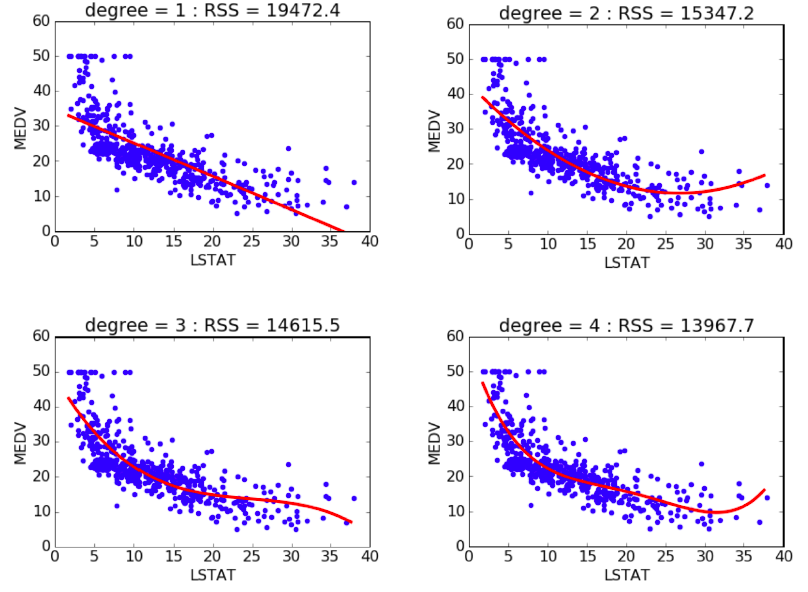
\includegraphics[width=.6\linewidth]{regression}
  \end{figure}

\subsection{Model evaluation}
Models should be evaluated on data \textbf{never seen before} during training : data must be split into \textbf{test and training set}.

\subsubsection{Hold out evaluation}
Reserves a certain amount for testing and the remainder for training:
\begin{itemize}
\item \textbf{too small} training sets might result in \textbf{poor} weight estimation
\item \textbf{too small} test sets might result in \textbf{poor} estimation of future predictions
\end{itemize}
For small unbalanced datasets,samples might not be representative.Also the selection of the right model degree could depend on the selected test set split.

\subsubsection{Cross-validation}
\begin{enumerate}
\item Split data into k subsets of \textbf{equal size}
\item Each subset is in turn used for testing and the remainder for training
\item The error estimates are averaged to yield an overall error estimate
\end{enumerate}
The subsets are often \textbf{stratified} to create homogeneous subgroups and reduce the variance.Usually \textbf{10-fold CV} is used as extensive experiments have shown that it is the best choice to get an accurate estimate.

\subsection{Overfitting}
Overfitting means learning the noise in data : good performance is achieved on training sets but bad performance on \textbf{test set}! This is often correlated to \textbf{large weight estimates} :  a good solution is to \textbf{penalize} large weights.

\subsubsection{Ridge Regression L2 Regularization}
Minimizes the cost function : 
$$ Cost(\overrightarrow{w}) = RSS(\overrightarrow{w})+ \alpha ||\overrightarrow{w}||^{2}_{2} = \sum \limits_{i=1}^{N} \left( y_i - \sum \limits_{j=0}^{D} w_jh_j(\overrightarrow{w_i}) \right)^2 + \alpha \sum \limits_{j=0}^{D}w^2_j$$
\begin{itemize}
\item $\alpha =0$ usual regression
\item $\alpha =\infty$ all weights = 0
\end{itemize}
Gradient descent becomes : 
$$ \Delta w_j= -2 \sum \limits_{i=0}^{N}h_j(\overrightarrow{x_i})(y_i- \hat{y_i}(\overrightarrow{w}^{(t)}))+2\alpha w_j$$
\begin{figure}[H]
  \centering
  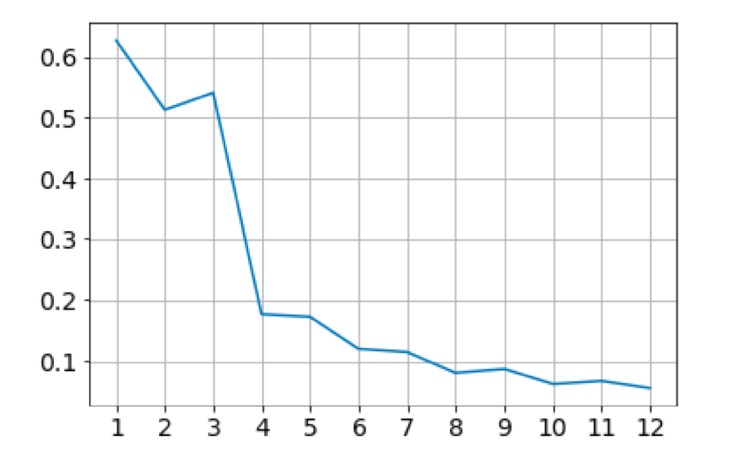
\includegraphics[width=.6\linewidth]{ridge1}
  \end{figure}
\begin{figure}[H]
  \centering
  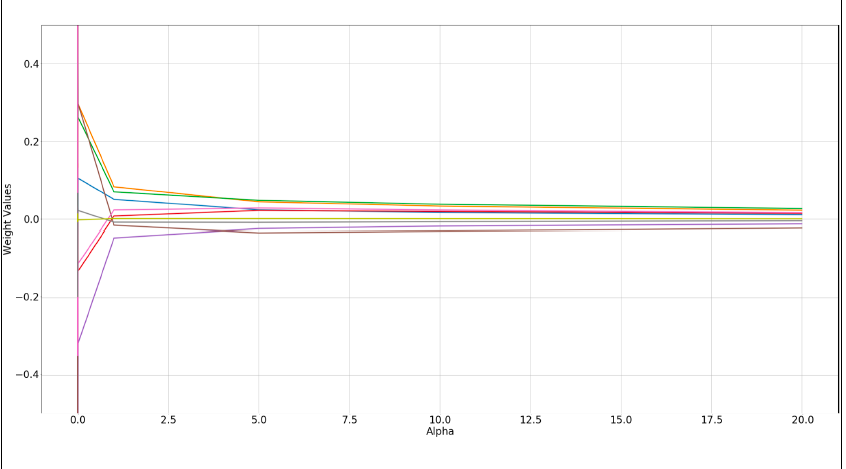
\includegraphics[width=.6\linewidth]{ridge2}
  \end{figure}

\subsubsection{Lasso Regression L1 Regularization}
Minimizes the cost function : 
$$ Cost(\overrightarrow{w}) = RSS(\overrightarrow{w})+ \alpha ||\overrightarrow{w}||_{1} = \sum \limits_{i=1}^{N} \left( y_i - \sum \limits_{j=0}^{D} w_jh_j(\overrightarrow{w_i}) \right)^2 + \alpha \sum \limits_{j=0}^{D}|w_j|$$
\begin{itemize}
\item $\alpha =0$ usual regression
\item $\alpha =\infty$ all weights = 0
\end{itemize}
Gradient descent becomes : 

\begin{figure}[H]
  \centering
  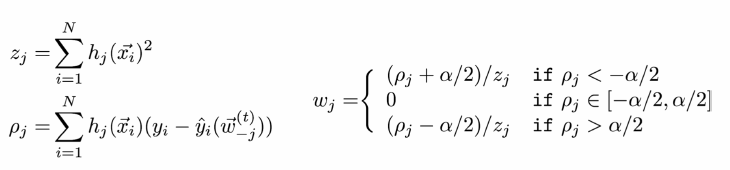
\includegraphics[width=.6\linewidth]{regressionlasso}
  \end{figure}

\begin{figure}[H]
  \centering
  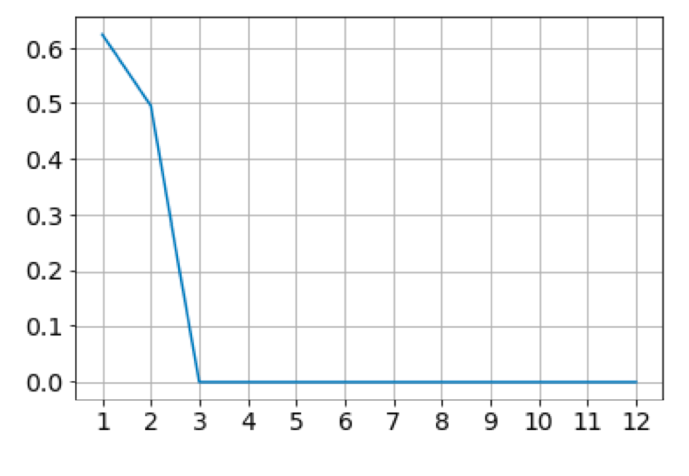
\includegraphics[width=.6\linewidth]{lasso1}
  \end{figure}

\begin{figure}[H]
  \centering
  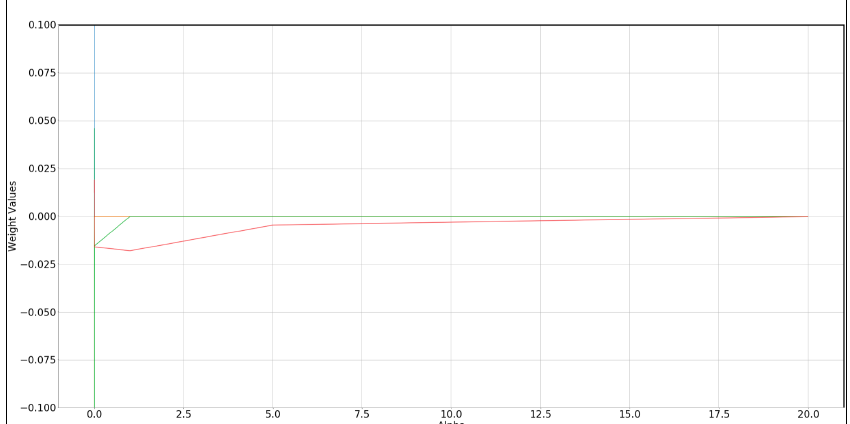
\includegraphics[width=.6\linewidth]{lasso2}
  \end{figure}
Lasso tends to \textbf{zero out less important feature} applying a so called \textbf{feature selection} which produces \textbf{sparser solutions}

\subsubsection{Alpha selection} 
The values of alpha should be selected using a \textbf{dev set} or \textbf{validation set} : a third set, different from test and training ,used to selected the right penalization parameter. The test set cannot be used since it using the selected alpha. The best solution is to split again the training set and obtain the validation set (if there is \textbf{enough data}).\\
If there is not enough data , $\alpha$ can be selected by applying k-fold cross-validation over the training data choosing $\alpha$ corresponding to the lowest average cost over k-fields.
  